\documentclass[11pt,a4paper]{article}
\usepackage[a4paper,top=2cm,bottom=2.2cm,left=2.3cm,right=2.3cm]{geometry}
\usepackage{mathptmx}
\usepackage[T1]{fontenc}
\usepackage[utf8]{inputenc}
\usepackage{enumitem}
\usepackage{tabularx}
\usepackage{array}
\usepackage[hidelinks]{hyperref}
\usepackage{xurl}
\usepackage{float}
\usepackage[font=small,labelfont=bf,skip=4pt]{caption}
\usepackage{tikz}
\usetikzlibrary{shapes.geometric,arrows.meta,positioning,fit,calc}
% Black-and-white methodology diagrams (TikZ)
\tikzset{
  box/.style={draw, rounded corners=2pt, align=center, font=\footnotesize, inner sep=3pt, minimum height=7mm},
  dbox/.style={box, double, double distance=1.2pt},
  dbx/.style={box, dashed},
  dec/.style={draw, diamond, aspect=2.2, align=center, font=\footnotesize, inner sep=1pt},
  db/.style={draw, cylinder, shape border rotate=90, aspect=0.22, align=center, font=\footnotesize, minimum height=11mm, inner sep=2pt},
  arr/.style={-{Stealth[length=2mm]}, thick},
  lab/.style={font=\scriptsize, fill=white, inner sep=1pt},
  note/.style={font=\scriptsize\itshape, align=center},
  cell/.style={draw, minimum width=17mm, minimum height=5.5mm, font=\scriptsize, inner sep=1pt},
}

% ---------- Figure: dataset preparation ----------
\newcommand{\figdata}{%
\begin{figure}[H]\centering
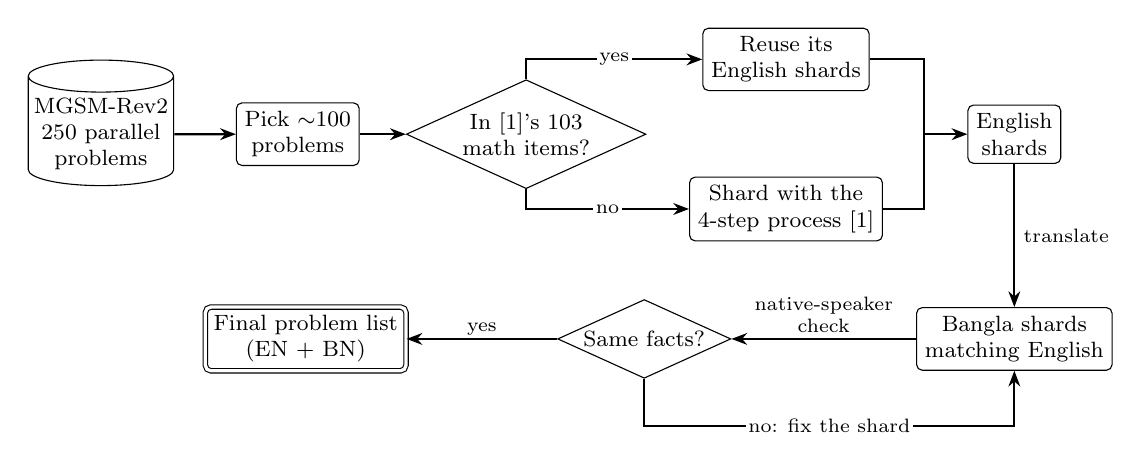
\begin{tikzpicture}
\node[db] (src) at (0,0) {MGSM-Rev2\\250 parallel\\problems};
\node[box] (pick) at (2.5,0) {Pick $\sim$100\\problems};
\node[dec] (ovl) at (5.4,0) {In [1]'s 103\\math items?};
\node[box] (reuse) at (8.7,0.95) {Reuse its\\English shards};
\node[box] (cut) at (8.7,-0.95) {Shard with the\\4-step process [1]};
\node[box] (en) at (11.6,0) {English\\shards};
\node[box] (bn) at (11.6,-2.6) {Bangla shards\\matching English};
\node[dec] (chk) at (6.9,-2.6) {Same facts?};
\node[dbox] (freeze) at (2.6,-2.6) {Final problem list\\(EN + BN)};
\draw[arr] (src) -- (pick);
\draw[arr] (pick) -- (ovl);
\draw[arr] (ovl.north) |- node[lab, pos=0.75] {yes} (reuse.west);
\draw[arr] (ovl.south) |- node[lab, pos=0.75] {no} (cut.west);
\draw[thick] (reuse.east) -| (10.45,0);
\draw[thick] (cut.east) -| (10.45,0);
\draw[arr] (10.45,0) -- (en.west);
\draw[arr] (en) -- node[lab, right=2pt, fill=none] {translate} (bn);
\draw[arr] (bn) -- node[lab, above=1pt, align=center, fill=none] {native-speaker\\check} (chk);
\draw[arr] (chk) -- node[lab, above] {yes} (freeze);
\draw[arr] (chk.south) |- ++(0,-0.25) -- ++(0,-0.35) -| node[lab, pos=0.25] {no: fix the shard} (bn.south);
\end{tikzpicture}
\caption{Dataset preparation. English shards are reused from [1] where possible; every Bangla shard is checked by hand before the problem list is fixed.}
\end{figure}}

% ---------- Figure: model selection ----------
\newcommand{\figmodels}{%
\begin{figure}[H]\centering
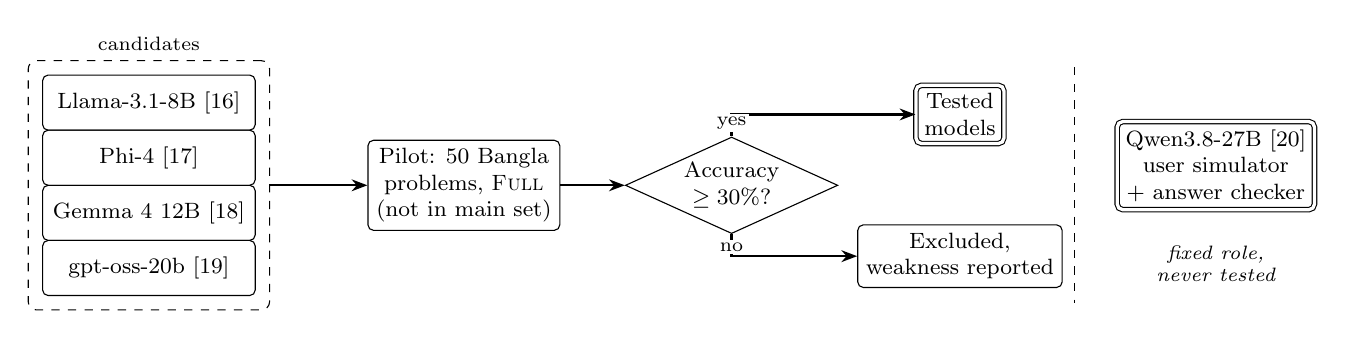
\begin{tikzpicture}
\node[box, minimum width=27mm] (m1) at (0,1.05) {Llama-3.1-8B [16]};
\node[box, minimum width=27mm] (m2) at (0,0.35) {Phi-4 [17]};
\node[box, minimum width=27mm] (m3) at (0,-0.35) {Gemma 4 12B [18]};
\node[box, minimum width=27mm] (m4) at (0,-1.05) {gpt-oss-20b [19]};
\node[draw, dashed, rounded corners=3pt, fit=(m1)(m4), inner sep=5pt, label={[font=\scriptsize]above:candidates}] (cand) {};
\node[box] (pilot) at (4.0,0) {Pilot: 50 Bangla\\problems, \textsc{Full}\\(not in main set)};
\node[dec] (pass) at (7.4,0) {Accuracy\\$\geq 30\%$?};
\node[dbox] (keep) at (10.3,0.9) {Tested\\models};
\node[box] (drop) at (10.3,-0.9) {Excluded,\\weakness reported};
\draw[arr] (cand) -- (pilot);
\draw[arr] (pilot) -- (pass);
\draw[arr] (pass.north) |- node[lab, pos=0.3] {yes} (keep.west);
\draw[arr] (pass.south) |- node[lab, pos=0.3] {no} (drop.west);
\draw[dashed] (11.75,1.5) -- (11.75,-1.5);
\node[dbox] (qwen) at (13.55,0.25) {Qwen3.8-27B [20]\\user simulator\\+ answer checker};
\node[note] at (13.55,-1.0) {fixed role,\\never tested};
\end{tikzpicture}
\caption{Model selection. Only candidates that pass the 30\% pilot cutoff are tested; the simulator model is kept separate from the tested models.}
\end{figure}}

% ---------- Figure: simulation ----------
\newcommand{\figsim}{%
\begin{figure}[H]\centering
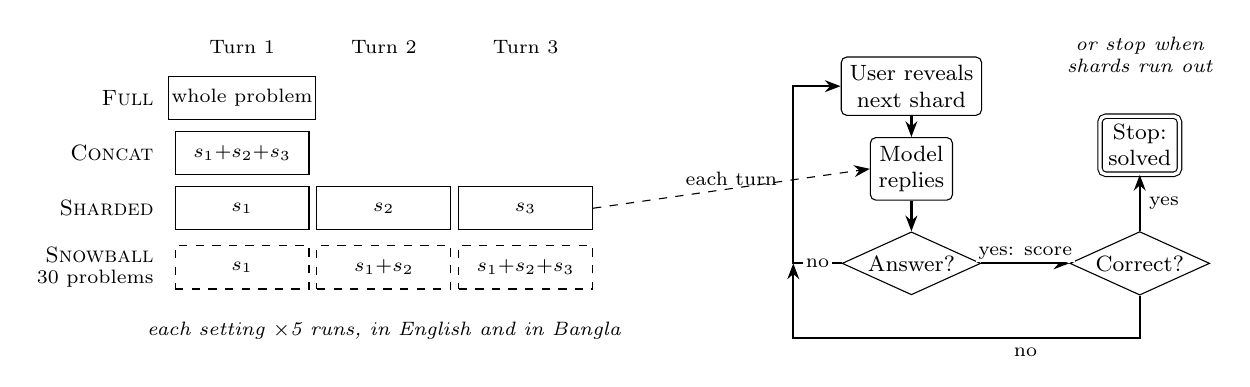
\begin{tikzpicture}
\foreach \i/\x in {1/2.5,2/4.3,3/6.1} \node[font=\scriptsize] at (\x,1.55) {Turn \i};
\node[font=\footnotesize, anchor=east] at (1.5,0.9) {\textsc{Full}};
\node[font=\footnotesize, anchor=east] at (1.5,0.2) {\textsc{Concat}};
\node[font=\footnotesize, anchor=east] at (1.5,-0.5) {\textsc{Sharded}};
\node[font=\footnotesize, anchor=east, align=right] at (1.5,-1.25) {\textsc{Snowball}\\[-2pt]{\scriptsize 30 problems}};
\node[cell] at (2.5,0.9) {whole problem};
\node[cell] at (2.5,0.2) {$s_1{+}s_2{+}s_3$};
\node[cell] at (2.5,-0.5) {$s_1$};
\node[cell] at (4.3,-0.5) {$s_2$};
\node[cell] (last) at (6.1,-0.5) {$s_3$};
\node[cell, dashed] at (2.5,-1.25) {$s_1$};
\node[cell, dashed] at (4.3,-1.25) {$s_1{+}s_2$};
\node[cell, dashed] at (6.1,-1.25) {$s_1{+}s_2{+}s_3$};
\node[note] at (4.3,-2.05) {each setting $\times$5 runs, in English and in Bangla};
% per-turn loop
\node[box] (rev) at (11.0,1.05) {User reveals\\next shard};
\node[box] (rep) at (11.0,0.0) {Model\\replies};
\node[dec] (ans) at (11.0,-1.2) {Answer?};
\node[dec] (cor) at (13.9,-1.2) {Correct?};
\node[dbox] (stop) at (13.9,0.3) {Stop:\\solved};
\draw[arr] (rev) -- (rep);
\draw[arr] (rep) -- (ans);
\draw[arr] (ans) -- node[lab, above] {yes: score} (cor);
\draw[arr] (cor) -- node[lab, right=2pt, fill=none] {yes} (stop);
\draw[arr] (ans.west) -| node[lab, pos=0.25] {no} (9.5,1.05) -- (rev.west);
\draw[arr] (cor.south) |- (9.5,-2.15) -- (9.5,-1.2);
\node[lab, fill=none] at (12.45,-2.33) {no};
\node[note] at (13.9,1.45) {or stop when\\shards run out};
\draw[dashed, -{Stealth[length=2mm]}] (last.east) -- node[lab, above, fill=none] {each turn} (rep.west);
\end{tikzpicture}
\caption{Simulation. Left: what the model sees in each turn ($s_i$ = shard $i$). Right: the loop run at every \textsc{Sharded} turn; the best attempt counts.}
\end{figure}}

% ---------- Figure: evaluation ----------
\newcommand{\figeval}{%
\begin{figure}[H]\centering
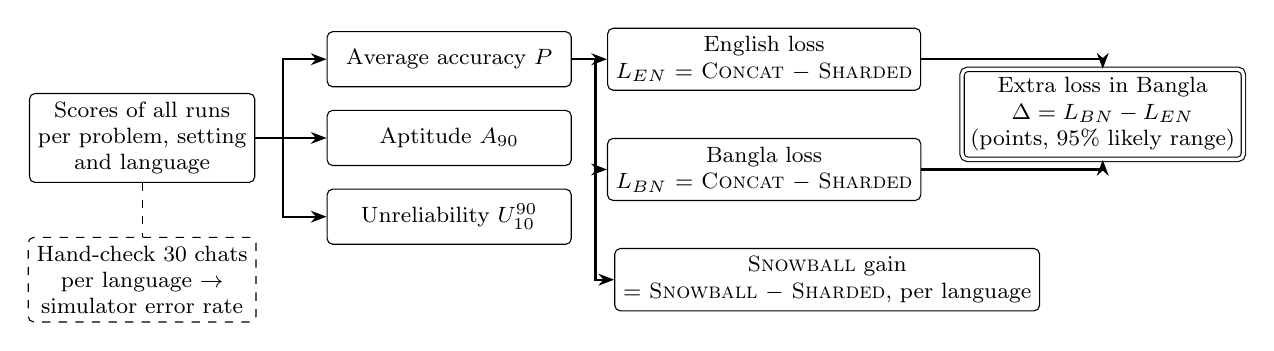
\begin{tikzpicture}
\node[box] (runs) at (0,0) {Scores of all runs\\per problem, setting\\and language};
\node[box, minimum width=31mm] (avg) at (3.9,1.0) {Average accuracy $P$};
\node[box, minimum width=31mm] (apt) at (3.9,0.0) {Aptitude $A_{90}$};
\node[box, minimum width=31mm] (unr) at (3.9,-1.0) {Unreliability $U_{10}^{90}$};
\node[box] (len) at (7.9,1.0) {English loss\\$L_{EN}$ = \textsc{Concat} $-$ \textsc{Sharded}};
\node[box] (lbn) at (7.9,-0.4) {Bangla loss\\$L_{BN}$ = \textsc{Concat} $-$ \textsc{Sharded}};
\node[dbox] (delta) at (12.2,0.3) {Extra loss in Bangla\\$\Delta = L_{BN} - L_{EN}$\\(points, 95\% likely range)};
\node[box] (snow) at (8.7,-1.8) {\textsc{Snowball} gain\\= \textsc{Snowball} $-$ \textsc{Sharded}, per language};
\node[dbx] (hand) at (0,-1.8) {Hand-check 30 chats\\per language $\to$\\simulator error rate};
\draw[dashed] (runs.south) -- (hand.north);
\draw[arr] (runs.east) -- ++(0.35,0) |- (avg.west);
\draw[arr] (runs.east) -- (apt.west);
\draw[arr] (runs.east) -- ++(0.35,0) |- (unr.west);
\draw[arr] (avg.east) -- ++(0.3,0) |- (len.west);
\draw[arr] (avg.east) -- ++(0.3,0) |- (lbn.west);
\draw[arr] (avg.east) -- ++(0.3,0) |- (snow.west);
\draw[arr] (len.east) -| (delta.north);
\draw[arr] (lbn.east) -| (delta.south);
\end{tikzpicture}
\caption{Evaluation. Each run is scored as in [1]; the main result $\Delta$ compares the loss from splitting in Bangla with the same loss in English.}
\end{figure}}

\setlength{\parindent}{0pt}
\setlength{\parskip}{6pt}
\pagestyle{plain}

% Numbered form item: \item{N}{Label}{optional note}
\newcommand{\formitem}[3]{%
  \par\vspace{4pt}\noindent\makebox[1.6em][l]{\textbf{#1.}}\textbf{#2}%
  \if\relax\detokenize{#3}\relax\else\ \textit{(#3)}\fi\par}
\newcommand{\blank}[1][4.5cm]{\underline{\makebox[#1][l]{}}}
\usepackage{needspace}
\setlength{\intextsep}{6pt plus 2pt minus 2pt}
\newcommand{\subhead}[1]{\par\needspace{3\baselineskip}\vspace{2pt}\textbf{#1}\par\vspace{-3pt}}

\begin{document}

\begin{center}
{\large\textbf{MILITARY INSTITUTE OF SCIENCE AND TECHNOLOGY, DHAKA}}\\[3pt]
\textbf{DEPARTMENT OF COMPUTER SCIENCE AND ENGINEERING}\\[3pt]
\underline{Application for the Approval of Course Project Research Proposal}\\[2pt]
\textit{Course: CSE 6701 Advanced Artificial Intelligence}
\end{center}

\hfill\textbf{Date of Application:} 21-11-2026

\formitem{1}{Name of the Students (Group 2):}{}
\begin{tabular}{@{\hspace{1.6em}}l l l}
(i) & Anika Ashraf & Roll No: 0424140025\\
(ii) & Faria Alam & Roll No: 1026140015\\
(iii) & Faysal Ahmed & Roll No: 0426140031\\
(iv) & Abrar Mahir Esam (Group Representative) & Roll No: 1025140022\\
(v) & Sachitra Halder & Roll No: 0426140027\\
(vi) & Muntasir Hasan Porag & Roll No: 0426140028
\end{tabular}

\formitem{2}{Contact Email (group representative):}{}
\hspace*{1.6em}Abrar Mahir Esam, abrarme118@gmail.com

\formitem{3}{Name of the Department:}{}
\hspace*{1.6em}Dept.\ of Computer Science and Engineering \hfill Program: M.Sc.Engg.\ (CSE)

\formitem{4}{Semester:}{}
\hspace*{1.6em}October 2026

\formitem{5}{Name of the Course Teacher:}{}
\hspace*{1.6em}Dr.\ Nusrat Sharmin, Associate Professor\\
\hspace*{1.6em}Affiliation: Department of Computer Science and Engineering, Military Institute of Science and Technology

\formitem{6}{Name of the Co-Supervisor:}{}
\hspace*{1.6em}Nil

\formitem{7}{Project Title:}{}
\hspace*{1.6em}\parbox[t]{\dimexpr\linewidth-1.6em}{\textbf{DO LLMS GET MORE LOST IN BANGLA? MULTI-TURN DEGRADATION ON PARALLEL ENGLISH--BANGLA MATH PROBLEMS}}

\formitem{8}{Background and Present State of the Problem:}{Not more than 350 words}

Large language models (LLMs) score well when a task arrives in one complete message, but real users often explain what they want bit by bit over several messages. Laban et al.\ [1] tested this directly. They cut tasks from well-known test sets into small pieces (``shards'') and had an AI, playing the user, reveal one piece per turn. Across 15 models and six tasks, scores dropped by 39\% on average. Best-case scores fell only 16\%, while the gap between good and bad runs rose by 112\%: models stayed capable but became unreliable, and once they took a wrong turn they rarely recovered.

Later work confirms that multi-turn conversation remains hard [2], [3]. Kami\'nski et al.\ [4] show that models can detect when information is missing but do not reliably act on it. Several methods reduce the drop, by extra training [5], [7], [8] or by rewriting the user's request [6]. All of them are tested in English only.

Work beyond English is limited. Pintor et al.\ [9] adapted the sharded setup to Filipino and tested two simple fixes: a closing summary turn (Recap) and repeating earlier pieces each turn (Snowball). Multi-IF [11] adds new instructions at each turn across eight languages, and Kim et al.\ [10] test how models react when the user switches language between turns; neither splits one fixed task into pieces.

For Bangla, single-message math is already well studied. MathMist [15] reports lower accuracy on Bangla than on English math. MGSM-Rev2 [14] corrects translation errors in MGSM [13], which was built from GSM8K [12], and shows that part of the earlier gap between languages came from those errors and from how answers were read.

No study yet shows whether splitting the same math problems across turns reduces accuracy \emph{more} in Bangla than in English, and whether an existing fix helps as much on matched Bangla problems as on English ones. A model that is simply weaker at Bangla is a different problem from one that also gets lost more easily in a Bangla conversation.

\formitem{9}{Objectives with Possible Outcome:}{Not more than 150 words}

\textbf{The objectives of this study are}
\begin{enumerate}[leftmargin=2em,itemsep=1pt,topsep=2pt]
\item To rerun the base paper's math test with free, open models on our own GPUs, with another open model playing the user and checking answers.
\item To build a matched English--Bangla set of sharded math problems, checked by native speakers.
\item To measure, in percentage points, whether splitting a problem across turns costs more accuracy in Bangla than in English, along with best-case score and consistency.
\item To test whether repeating earlier pieces each turn (\textsc{Snowball}) gives a larger or smaller accuracy gain over \textsc{Sharded} in Bangla than in English.
\end{enumerate}

\textbf{The expected outcomes of this study are}
\begin{enumerate}[leftmargin=2em,itemsep=1pt,topsep=2pt]
\item A released English--Bangla sharded math dataset of about 100 problems.
\item A measurement of the extra loss in Bangla, which may be zero.
\item A full paper submitted to the Third Workshop on Bangla Language Processing (BLP 2027, co-located with NAACL 2027), under the topic Resources, Evaluation, and Efficient NLP.
\end{enumerate}

\formitem{10}{Outline of Methodology/Experimental Design:}{Not more than 300 words}

We reuse the math setup and code of [1], [21] on matched English--Bangla problems. Only the language, models, user and checker change.

\subhead{Dataset Preparation:}
About 100 problems come from MGSM-Rev2 [14] (CC BY-SA 4.0; 250 GSM8K [12] problems in 11 languages). We reuse [1]'s English shards where it already split a problem (App.~J.4), after checking them against Rev2, and split the rest the same way. Native speakers check each Bangla shard against its English partner. The problem list is then fixed.
\figdata

\subhead{Model Selection:}
Candidates are Llama-3.1-8B-Instruct [16] and Phi-4 [17], both in [1], plus the newer Gemma~4 12B [18] and gpt-oss-20b [19]. A model is kept only if it solves at least 30\% of a separate 50-problem Bangla pilot (\textsc{Full}). Below 30\%, a model has little room to drop, so any loss would be hidden. Qwen3.8-27B [20] (thinking off) plays the user and checks answers; it is never tested.
\figmodels

\subhead{Simulation:}
Each problem runs 5 times per language: whole problem in one message (\textsc{Full}), all shards in one message (\textsc{Concat}), one shard per turn (\textsc{Sharded}). As in [1], shard 1 comes first and the simulator picks the next shard; we log the order. The checker marks the final number right only if it equals the answer (Bangla digits read as 0--9). Chats end on a correct answer or when shards run out. \textsc{Snowball} runs on 30 problems in both languages.
\figsim

\subhead{Evaluation and Analysis:}
We report average accuracy, best-case score (aptitude) and the gap between good and bad runs (unreliability) per setting and language [1, \S4.2]. The main result is Bangla's extra loss, in points: (\textsc{Concat} $-$ \textsc{Sharded}) in Bangla minus the same in English. Its 95\% likely range comes from re-sampling problems (bootstrap). For \textsc{Snowball} we report its gain over \textsc{Sharded} per language. We hand-check 30 conversations per language.
\figeval

\formitem{11}{References:}{}
\begin{enumerate}[label={\arabic*.},leftmargin=2em,itemsep=1pt,topsep=2pt]\small\raggedright
\item P. Laban, H. Hayashi, Y. Zhou and J. Neville, ``LLMs Get Lost in Multi-Turn Conversation,'' in \textit{Proc. Int. Conf. Learning Representations (ICLR)}, 2026.
\item Y. Li, X. Shen, X. Yao, X. Ding, Y. Miao, R. Krishnan and R. Padman, ``Beyond Single-Turn: A Survey on Multi-Turn Interactions with Large Language Models,'' \textit{Trans. Mach. Learn. Res. (TMLR)}, 2026.
\item K. Deshpande, V. Sirdeshmukh \textit{et al.}, ``MultiChallenge: A Realistic Multi-Turn Conversation Evaluation Benchmark Challenging to Frontier LLMs,'' in \textit{Findings of the Assoc. Comput. Linguistics: ACL}, Vienna, Austria, 2025, pp. 18632--18702.
\item J. Kami\'nski \textit{et al.}, ``Knowing When Not to Answer: Cross-Domain and Multi-Turn Generalization of Latent Underspecification Signals,'' arXiv:2610.08413, 2026.
\item M. Li \textit{et al.}, ``Mitigating Lost in Multi-turn Conversation via Curriculum RL with Verifiable Accuracy and Abstention Rewards,'' in \textit{Proc. 64th Annu. Meeting Assoc. Comput. Linguistics (ACL)}, San Diego, CA, USA, 2026, pp. 33364--33381.
\item G. Liu, F. Zhu, R. Feng, C. Ma, S. Wang and G. Meng, ``Intent Mismatch Causes LLMs to Get Lost in Multi-Turn Conversation,'' arXiv:2602.07338, 2026.
\item T. Chen, S. Wu and J. Leskovec, ``Found in Conversation: LLMs Teach Themselves to Close the Multi-Turn Gap,'' in \textit{Advances in Neural Information Processing Systems (NeurIPS)}, 2026.
\item H. Zheng \textit{et al.}, ``MAIGO: Mitigating Lost-in-Conversation with History-Cleaned On-Policy Self-Distillation,'' arXiv:2605.27186, 2026.
\item R. R. Pintor, L. J. Wang and G. Pepito, ``Evaluating Large Language Models in Filipino Underspecified, Multi-Turn Conversations,'' in \textit{Proc. 26th Philippine Computing Science Congress (PCSC)}, 2026.
\item K. Kim, C. Li Chen and A. Sotnikova, ``Query-Following vs Context-Anchoring: How LLMs Handle Cross-Turn Language Switching,'' in \textit{Proc. 1st Workshop on Multilingual Multicultural Evaluation}, 2026, pp. 196--203.
\item Y. He \textit{et al.}, ``Multi-IF: Benchmarking LLMs on Multi-Turn and Multilingual Instructions Following,'' arXiv:2410.15553, 2024.
\item K. Cobbe \textit{et al.}, ``Training Verifiers to Solve Math Word Problems,'' arXiv:2110.14168, 2021.
\item F. Shi \textit{et al.}, ``Language Models are Multilingual Chain-of-Thought Reasoners,'' in \textit{Proc. Int. Conf. Learning Representations (ICLR)}, 2023.
\item J.-T. Peter, D. Vilar, T. Domhan, D. Malkin and M. Freitag, ``Mind the Gap\ldots\ or Not? How Translation Errors and Evaluation Details Skew Multilingual Results,'' in \textit{Proc. 5th Workshop on Generation, Evaluation and Metrics (GEM)}, 2026, pp. 191--204.
\item M. E. Sobhani, M. F. A. Sayeedi, T. Mohiuddin, M. M. Islam and S. Shatabda, ``MathMist: A Parallel Multilingual Benchmark Dataset for Mathematical Problem Solving and Reasoning,'' in \textit{Findings of the Assoc. Comput. Linguistics: EACL}, Rabat, Morocco, 2026, pp. 2524--2550.
\item A. Grattafiori \textit{et al.}, ``The Llama 3 Herd of Models,'' arXiv:2407.21783, 2024.
\item M. Abdin \textit{et al.}, ``Phi-4 Technical Report,'' arXiv:2412.08905, 2024.
\item Gemma Team, Google DeepMind, ``Gemma 4 Technical Report,'' arXiv:2607.02770, 2026.
\item OpenAI, ``gpt-oss-120b \& gpt-oss-20b Model Card,'' arXiv:2508.10925, 2025.
\item Qwen Team, ``Qwen3.8-27B,'' model card, Hugging Face, 2026. [Online]. Available: \url{https://huggingface.co/Qwen/Qwen3.8-27B}
\item Microsoft, ``lost\_in\_conversation: Code and Data for LLMs Get Lost in Multi-Turn Conversation,'' GitHub repository, 2025. [Online]. Available: \url{https://github.com/microsoft/lost_in_conversation}
\end{enumerate}

\end{document}
